\documentclass[runningheads,a4paper]{llncs}%
%\documentclass[runningheads,a4paper]{article}%
%
\usepackage{amssymb}%
\usepackage{amsmath}%
\setcounter{tocdepth}{3}%
\usepackage{graphicx}%
\usepackage{listings}
\usepackage{lstlangampl}
\usepackage{algorithm}
\usepackage{algpseudocode}
\usepackage{pgfplots}
\pgfplotsset{compat=1.9}
%
\usepackage{url}%
\urldef{\mailsa}\path|{felix.kurth, schupp}@tu-harburg.de|%
\urldef{\mailsb}\path|stephan.weissleder@gmail.com|%
\newcommand{\keywords}[1]{\par\addvspace\baselineskip%
\noindent\keywordname\enspace\ignorespaces#1}%
%
% My user defined inclues%
\usepackage{color} %Makes incscape pdf_tex work%
\usepackage[T1]{fontenc} % makes Guillemont available%
\newcommand{\UMLType}[1]{\textsf{\textit{#1}}} %
\newcommand{\TCGType}[1]{#1}%
\newcommand{\UMLReference}[1]{\textsf{\textit{#1}}} %
\newcommand{\AMPLCode}[1]{\texttt{#1}}
\newcommand{\OCLCode}[1]{\texttt{#1}}
\newcommand{\OCLVar}[1]{\textit{#1}}
\newcommand{\AlgDataType}[1]{\textsf{#1}}

\newcommand{\AMPLListing}[1]{\begin{lstlisting}[basicstyle=\ttfamily\scriptsize,language=ampl]{#1}\end{lstlisting}}
%
\begin{document}%
%
\mainmatter  % start of an individual contribution%
%
% first the title is needed%
\title{Generating Test Data from a UML Activity using the AMPL Interface for Constraint Solvers}%
%\title{Automated Generation of Unit Tests from UML Activity Diagrams using the AMPL Interface for Constraint Solvers}%
%
% a short form should be given in case it is too long for the running head%
\titlerunning{Automated Generation of Test Data}%
%
% the name(s) of the author(s) follow(s) next%
%
% NB: Chinese authors should write their first names(s) in front of%
% their surnames. This ensures that the names appear correctly in%
% the running heads and the author index.%
%
\author{Felix Kurth\inst{1}%
% \thanks{Please note that the LNCS Editorial assumes that all authors have used%
% the western naming convention, with given names preceding surnames. This determines%
% the structure of the names in the running heads and the author index.}%
\and Sibylle Schupp\inst{1}%
%
\and Stephan Wei{\ss}leder\inst{2}
%\thanks{Affiliations?}
}%
%
%\authorrunning{Lecture Notes in Computer Science: Authors' Instructions}%
% (feature abused for this document to repeat the title also on left hand pages)%
%
% the affiliations are given next; don't give your e-mail address%
% unless you accept that it will be published%
\institute{Hamburg University of Technology, Institute for Software Systems,\\%
Schwarzenbergstr. 95, 21073 Hamburg, Germany\\%
\mailsa\\%
\url{http://www.sts.tu-harburg.de}
\and
\mailsb\\
\url{www.model-based-testing.de/person/stephan_weissleder}}%
%
%
% NB: a more complex sample for affiliations and the mapping to the%
% corresponding authors can be found in the file "llncs.dem"%
% (search for the string "\mainmatter" where a contribution starts).%
% "llncs.dem" accompanies the document class "llncs.cls".%
%
%
%\toctitle{Lecture Notes in Computer Science}%
%\tocauthor{Authors' Instructions}%
\maketitle%
%
\begin{abstract}%
Testing is one of the most wide-spread means for quality assurance. Modelling and
automated test design are two means to improve effectivity and efficiency of
testing. In this paper, we present a method to generate test data from UML
activity diagrams and OCL constraints by combining symbolic execution and
state--of--the--art constraint solvers. Our corresponding prototype
implementation is integrated in the existing test generator ParTeG and generates
C++ unit tests.
Our key improvement is the transparent use of multiple industry strength solvers
through a common interface; this allows the user to choose between an expressive
constraint language or highly optimised test data generation. We use infeasible
path elimination to improve the performance of test generation and boundary
value analysis to improve the quality of the generated test data. We provide an
industrial case study and measure the performance of our tool using different
solvers in several scenarios.
%and boundary value analysis
%We present a method to generate test data from UML activity diagrams. Our method uses symbolic execution to collect embedded OCL constraints along a control flow and we derive test data using state--of--the--art constraint solvers. The generated tests will satisfy control flow--based coverage criteria on the used models. We also use boundary value analysis for testing. A special focus is on allowing mixed integer non--linear programming as well as logical formulas in OCL constraints. The presented method has been implemented in a demo Eclipse plug--in that generates fully automatically compilable C++ unit tests from activity diagrams. We report on an industrial case study with our tool.%
%\keywords{Model--Based Testing, Activity Diagram, AMPL, Constraint Solving, Mixed Integer Non--Linear Programming, Symbolic Execution, Boundary Value Analysis, Eclipse Plug--In, Case Study}%
\keywords{Model--Based Testing, Activity Diagram, AMPL, Constraint Solving, Infeasible Path Elimination, Boundary Value Analysis, Mixed Integer Non--Linear Programming}%
\end{abstract}%
\section{Introduction}%
Model--Based Engineering is a promising technology for system engineering.
The Unified Modelling Language\textsuperscript{\texttrademark} (UML) is the quasi
standard for model--based specifications. A UML activity diagram can be used to
give a quick and intuitive overview of a
system. It can also be used to formally describe details of a procedural
implementation. They can be refined in a step-wise manner starting with a vague description of the intended system usage and adding more details later on.

Modelling is not an end in itself.
The benefits of Model--Based Engineering are automated subsequent tasks
in software development like, e.g., testing. We want to automatically generate test
data from an activity diagram with embedded constraints described using the Object Constraint Language (OCL). 
The test model describes the relevant control flows in the system under test
(SUT). The embedded OCL constraints describe interdependencies between the
variables and how variables change their value.

In this paper we present a transformation from an activity diagram into an `A
Mathematical Programming Language' (AMPL) program. For that, we symbolically
execute control flow paths in the activity diagram and encode each of them as
AMPL programs. The solutions of these resulting AMPL programs contain input
values and corresponding oracle values that can be used to test the
implementation. Since test data at the boundaries of path constraints has a
higher probability to detect failures, we also integrate boundary value analysis
in test generation. Depth--first search is used to find control flow paths and
we introduced \emph{early infeasible path elimination} within the depth--first
search to reduce the runtime of our algorithm. The presented transformation is
implemented as part of a master thesis~\cite{Kurth2014AutomatedGen} in a
proof of concept fully automated unit test generation tool called Activity
Tester (AcT). The tool is integrated as a feature into the Partition
Test Generator (ParTeG) available as Eclipse plug--in~\cite{PartegWebsite}.

The paper is structured as follows. Section~\ref{sec:LiteratureReview}
contains the related work. An introduction to AMPL and the used models
is given in Section~\ref{sec:Preliminaries}. 
Section~\ref{sec:Algorithm} contains a description of the core ideas of the
proposed algorithm. The report on our case study is given in
Section~\ref{sec:results}. The paper is concluded in Section~\ref{sec:Recommendation}.

\section{Related Work}%
\label{sec:LiteratureReview}%
%While it is very common to use state machines as the test model, less research
%is performed on generating tests from UML activity diagrams. 
There are several approaches for test generation based on activity diagrams.
For instance, Wang Linzhang et
al. propose in~\cite{Linzhang04GeneratingTestCasefromActivityGrayBoxMethod} a
path--search--based method to find test scenarios in an activity diagram.
They implemented the proof--of--concept tool UMLTGF. 
Minsong et al.~\cite{mingsong2006automatic} propose to randomly
generate Java unit tests and match the test execution traces to the control flow paths 
in the activity diagram. They then select a subset from the test cases that
covers all simple paths in the test model. Our method is also
path--search--based like
~\cite{Linzhang04GeneratingTestCasefromActivityGrayBoxMethod} and unlike
~\cite{mingsong2006automatic} we are using constraint solvers to find test data.

Wei{\ss}leder and Sokenou presented a data--oriented approach to
select test cases~\cite{weissleder2008automatic}. They use abstract
interpretation to derive partitions and corresponding boundaries of the domain of input values. 
Wei{\ss}leder~\cite{ParTeG} describes a detailed collection of
different model--based structure- and data--oriented coverage criteria including their formal definition.
The source code of ParTeG, the proof--of--concept tool associated with this thesis, is
freely available~\cite{PartegWebsite}. It uses graph search in combination with
abstract interpretation and a comprehensive framework, allowing the user to
steer which coverage criteria the generated test cases will adhere to. In
contrast to the data--oriented test data generation with abstract interpretation
we are using symbolic execution. We are also offering boundary value analysis
based on mathematical optimisation instead of data--partitions.

%Using OCL as input and trying to obtain test data by solving OCL constraints
%there have been several proposals on how exactly to find models that make an OCL
%formula true. 
There are several approaches to integrate the solution of OCL formulas.
Ali et al.~\cite{ali2011search} use
evolutionary algorithms to search for potential solutions of OCL
constraints. Krieger and Knapp~\cite{krieger2008executingUnderspecifiedOCL} use a SAT solver to find
instantiations of variables satisfying OCL constraints. They 
transform OCL formulas into boolean formulas and use a SAT-solver-based model finderfor solving these formulas.
In contrast, we generate models for OCL formulas not based on a single
heuristic or a single solver, but we are using the AMPL frontend to which we can
link either a heuristic or an algorithm.

Malburg and Fraser~\cite{malburg2011combining} propose a hybrid
approach. On the top level they use a genetic algorithm evolving a population of
candidate test data. Internally, they provide guidance to the genetic algorithm
by providing a special mutation operator performing dynamic symbolic execution.
Also the white--box unit test tool PEX~\cite{pex} from
Microsoft\textsuperscript{\textregistered} research is based on dynamic symbolic
execution. Both~\cite{malburg2011combining} and~\cite{pex}
execute the implementation with random input values and generate new
input values by collecting path conditions along the executed control flow.
Then they negate one of the path conditions and use a constraint solver to find
a solution. 
%The generated solution yields new input data, which is guaranteed to take another control flow path in the program. 
Like the presented work, we also use symbolic execution.
Since we are only performing a static analysis, however, we do not need the source code to generate test cases. 
So in contrast to the related work, our tool is also suitable for black--box testing.

\section{Preliminaries}%
\label{sec:Preliminaries}
In this section, we introduce the programming language AMPL and the semantics of
the used test models.
\subsection{AMPL and its Solvers}%
\label{sec:AMPL}%
We use `A Mathematical Programming Language' (AMPL) by Robert Fourer~\cite{AMPL}
to formalise the execution of a control flow path in the test model.
In this section, we describe AMPL and introduce the
solvers we have used to generate test data.
AMPL can be used to state linear, non--linear, and logical constraints. Variables can
be continuous or discrete. The AMPL system serves as a common interface to a
variety of solvers. Depending on the constraint satisfaction problem encoded in
the AMPL program a suitable solver can be selected to solve the problem. If all
\begin{table}[hb]%
\begin{center}%
\begin{tabular}{l r r r r r r r r}%
Solver                         & MILP       & NLP        & SMT        & MINLP\\%
\hline%
Cplex                          & \checkmark &            &            &\\%
LPsolve\cite{lpsolve}          & \checkmark &            &            &\\%
Gurobi                         &            & \checkmark &            &\\%
Minos                          &            & \checkmark &            &\\%
IlogCP\cite{ilogcp}            & \checkmark &            & \checkmark &\\%
GeCoDE\cite{gecode}            &            &            & \checkmark &\\%
Couenne\cite{Belotti09couenne} & \checkmark & \checkmark &            & \checkmark\\%
\hline%
\end{tabular}%
\end{center}%
\caption{List of solvers and problems they can solve.}%
\label{tab:Solvers}%
\end{table}
constraints are linear we use a solver that is specialized on mixed integer
linear programming (MILP), for example, Cplex or LPsolve~\cite{lpsolve}. If
constraints are non--linear but convex and all variables are continuous we use a
non--linear programming (NLP) solver. For problems with non--linear constraints
and discrete as well as continuous variables we need a solver capable of solving
mixed integer non--linear programming (MINLP), for example,
Couenne~\cite{Belotti09couenne}. If logical operations are used in the
constraints, a satisfiability modulo theories (SMT) solver supporting
appropriate background theories is used, for example, GeCoDE~\cite{gecode} or
IlogCP~\cite{ilogcp}. In Table~\ref{tab:Solvers} we show a selection of solvers
interfacing with AMPL. A checkmark in a cell means that we have successfully
tested the solver in the row on the problem named in the column.%

\subsection{Semantics of the Test Models}%
\label{sec:TestModel}%
For the transformation into `A Mathematical Programming Language' (AMPL)
presented in Section~\ref{sec:AMPLTransformation} we clarify the semantics of
the expected input model. Modelling elements of the UML such as
\UMLType{Activity} and UML references \UMLReference{name} or
\UMLReference{ownedParameter} are typeset in a special font. In this section, we
first detail which UML modelling elements we use and will then shortly
recapitulate the Petri--Net semantics of activity diagrams
(see~\cite{UML23Superstructure}). Further, we introduce the notion of a
\emph{state}, which will be relevant for our algorithm.

As test model we assume an activity diagram with \UMLType{Action}s,
\UMLType{ControlNode}s, and \UMLType{ControlFlow}s modelling the control flow of
an \UMLType{Operation}. The \UMLType{Activity} is linked as
\UMLReference{method} to its specifying \UMLType{Operation}. Each
\UMLType{Action} can contain several textual OCL constraints as
\UMLReference{localPostcondition} and each \UMLType{ControlFlow} can hold a
textual OCL constraint as \UMLReference{guard}. The textual OCL in the
\UMLReference{guard} and \UMLReference{localPostcondition} will be parsed in the
context of the specifying \UMLType{Operation}. That means the OCL constraints
can access all \UMLReference{ownedAttribute}s of the \UMLType{Class} containing
the specifying \UMLType{Operation}. Further, all \UMLReference{ownedParameter}s
of the specifying \UMLType{Operation} can be referenced in the textual OCL. We
interpret every \UMLType{Property} as variable that can change its value during
the execution of an \UMLType{Action}. A \UMLType{Parameter} will be interpreted
as a parameter that can not change its value during the execution of an
\UMLType{Action}.

When executing a control flow path, we start with a token in the
\UMLType{InitialNode}. We allow only one \UMLType{InitialNode} per
\UMLType{Activity}. The token can move along an enabled \UMLType{ControlFlow}. A
\UMLType{ControlFlow} is enabled when the OCL constraint in its
\UMLReference{guard} evaluates to true. We say that an \UMLType{Action} is being
executed when a token resides in the \UMLType{Action}.

We refer to an assignment of all variables and parameters as \emph{state}. While
the token resides in the \UMLType{InitialNode} there is an initial state. After
each execution of an \UMLType{Action} the current state can change according to
the OCL constraints contained in the \UMLType{Action}'s
\UMLReference{localPostcondition}. An OCL constraint contained as
\UMLType{localPostcondition} can specify a relation between the current state
and the previous state. Consequently, the states are interconnected with each
other via \UMLReference{localPostcondition}s. The set of all relations contained
in \UMLType{localPostcondition}s can be seen as state transition function. For a
\UMLType{ControlFlow} to be enabled the OCL constraint in its
\UMLReference{guard} has to evaluate to true with respect to the current state.
OCL constraints contained in a \UMLReference{guard} can only specify a relation
between the variables and parameters within a single state. It is not possible
to access the value of a variable in the previous state within a
\UMLReference{guard}.
\section{The Algorithm}%
\label{sec:Algorithm}%
In this section we explain the core ideas of the algorithm that we implemented
in the tool available from~\cite{PartegWebsite}. First, we demonstrate with a
small example how the execution of a control flow path can be formalised. Then
we show how to acquire test data that is at the boundary of path constraints
and, finally, we present an algorithm that efficiently searches for executable
control flow paths.%
\subsection{Overview}%
Symbolic execution is done by transforming an activity diagram into a
parameterised AMPL model representing all relevant OCL Constraints,
\UMLType{Properties} , and \UMLType{Parameter}s. This transformation preserves
the original semantics of the activity diagram.

The parameters of the AMPL model encode a control flow path. An assignment of
each variable in each state is generated by state--of--the--art constraint
solvers from an AMPL model with given parameters. The generated variable
assignment is suitable test data. A great advantage of a commonly used
mathematical programming language is that industrial--strength solvers are
available for a wide variety of problems (see Section~\ref{sec:AMPL}).
\subsection{AMPL Transformation}%
\label{sec:AMPLTransformation}%
\begin{figure}%
\def\svgwidth{\textwidth}%
\graphicspath{{./pics/}}%
\input{./pics/AssignmentDecision.pdf_tex}%
\caption{A simple UML activity diagram}%
\label{fig:AssignmentDecision}%
\end{figure}%
An AMPL model encodes the relevant \UMLType{Properties}, \UMLType{Parameter}s, and OCL constraints
contained in an activity diagram. We call a sequence of
\UMLReference{ControlFlow}s \emph{control flow path}. For two subsequent
\UMLType{ControlFlow}s A and B in a control flow path it holds that
A.target=B.source. A control flow path is encoded in the AMPL data.

We model the execution of a control flow path as a series of states. Each AMPL
model has one parameter called \AMPLCode{pathlength} representing the number of
\UMLType{Action}s on a control flow path. Executing an \UMLType{Action} changes
the state, consequently, there are \AMPLCode{pathlength + 1} states. Since a
\UMLType{Property} can have a distinct value in each state, they are modelled as
an array of variables. \UMLType{Parameter}s are constant and are therefore
represented by a single AMPL variable. Every \UMLType{Property} and
\UMLType{Parameter} has either integer, float, or boolean as
\UMLReference{type}; in AMPL we specify the domain of an AMPL variable
correspondingly.

The OCL constraints in Figure~\ref{fig:AssignmentDecision} reference three
different OCL variables. We assume $a$ and $returnValue$ to be
\UMLType{Parameter}s that are modelled as a single variable in AMPL and we
assume $x$ to be a \UMLType{Property} that is modelled as an array of variables.
We further assume that all three UML elements have the \UMLReference{type}
integer. Consequently, we generate the following AMPL code for them: %
\begin{lstlisting}[basicstyle=\ttfamily,language=ampl]
var a : integer;
var returnValue : integer;
var x{0..pathlength} : integer;
\end{lstlisting}%
% The underlying MOF Model--to--Text Transformation Language (MOFM2T) template~\cite{m2t.standard}, generating AMPL code from a \UMLType{Parameter} or \UMLType{Property} is shown in Algorithm~\ref{alg:m2tvariable}.
% \begin{algorithm}
% \begin{lstlisting}[escapeinside={@}{@},breaklines=true]
% [@\bfseries{template}@ public VariableToAMPL(var : @\UMLType{TypedElement}@)]
%   [@\bfseries{let}@ type : @\UMLType{PrimitiveType} = var.type@]
%     var [var.name/] [@\bfseries{if}@ var.oclIsKindOf(@\UMLType{Property}@)] {0..pathlength} [/@\bfseries{if}@][Type2AMPL(type)/] :=1;
%   [/@\bfseries{let}@]
% [/@\bfseries{template}@]
% [@\bfseries{template}@ public Type2AMPL(type : @\UMLType{PrimitiveType}@)]
%   [@\bfseries{if}@ type.name = 'integer'] : integer >=-10000, <= 10000 [/@\bfseries{if}@]
%   [@\bfseries{if}@ type.name = 'boolean'] in 0..1 [/@\bfseries{if}@]
%   [@\bfseries{if}@ type.name = 'real'] >=-10000, <= 10000 [/@\bfseries{if}@]
% [/@\bfseries{template}@]
% \end{lstlisting}%
% \caption{Model--to--text transformation from \UMLType{Property} or \UMLType{Parameter} to AMPL model}%
% \label{alg:m2tvariable}%
% \end{algorithm}

During execution, a \UMLType{ControlFlow}'s \UMLReference{guard} or an
\UMLType{Action}'s \UMLReference{localPostcondition} is always evaluated with
respect to the current state. The set of states in which an \UMLType{Action} or
\UMLType{ControlFlow} is being executed is called \emph{activation set}. There
is one activation set for each \UMLType{ControlFlow} having an OCL
\UMLReference{guard} and each \UMLType{Action} having an OCL
\UMLReference{localPostcondition}. All OCL \UMLReference{localPostcondition}s
and OCL \UMLReference{guard}s are contained in the AMPL model as constraints,
which can be switched on and off for each state. In the AMPL model states are
referenced via their index. For each \UMLType{Action} and \UMLType{ControlFlow}
the activation set is declared as a subset of the set
\AMPLCode{\{0..pathlength\}}. Each OCL constraint in a \UMLReference{guard} or
\UMLReference{localPostcondition} is transformed into an indexed collection of
constraints over the activation set.

If the variable reference was marked with \verb=@pre= we are accessing the
variable in the previous state and thus need to subtract one from the index;
otherwise we access the variable at the index from the activation set. The AMPL
model code generated for the Assignment \UMLType{Action} in
Figure~\ref{fig:AssignmentDecision} is, for example, as follows:%
\begin{lstlisting}[basicstyle=\ttfamily,language=ampl,breaklines=true]
set Assignment within {0..pathlength} default {};
s.t. Assignment_post0 {i in Assignment} : a*x[i]=2*x[i-1]*x[i-1]-3;
\end{lstlisting}
The value of the parameter \AMPLCode{pathlength} as well as the elements of each
activation set will be specified in the AMPL data. This way, there is one AMPL
model per activity diagram and any control flow path within the activity diagram
can be specified in the AMPL data. Let us, for example, encode the bold printed
control flow path from Figure~\ref{fig:AssignmentDecision} as AMPL data. Starting at the
\UMLType{InitialNode}, the current state is the initial state with the index
$0$. In this state there are no constraints. When we reach the Assignment
\UMLType{Action} our current state switches to $1$. Since there is a
post--condition for Assignment, we add $1$ to the activation set of the
Assignment. The next \UMLType{ControlFlow} has an OCL guard, consequently we add
$1$ to its activation set. Further, we add $2$ to the activation set of the Then
\UMLType{Action}. In AMPL syntax, the data specifying this path is:%
\begin{lstlisting}[basicstyle=\ttfamily,language=ampl]
param pathlength := 2;
set Assignment := 1;
set Cf_Then := 1;
set Then := 2;
\end{lstlisting}%
% The transformation from a sequence of \UMLType{ControlFlow}s into a map of activation sets is given in Algorithm~\ref{alg:ActivationSet}.%
% \begin{algorithm}
% \begin{algorithmic}
% \Require path := sequence of \UMLType{ControlFlow}s
% \Ensure activationSets contains activation sets representing the given path
% \State activationSets(element : \UMLType{NamedElement}) : Integer Set \Comment Mapping from an UML element to a set of integers. Initially all sets are empty.
% \State i : integer $\gets$ 0 \Comment index of the current state
% \ForAll{cf : \UMLType{ControlFlow} $\in$ path}
% \If{ cf.guard != null}
% \State activationSet(cf).add(i)
% \EndIf
% \If{ cf.target.oclIsKindOf(\UMLType{Action}) }
% \State i $\gets$ i+1 \Comment state changes
% \State activationSet(cf.target).add(i)
% \EndIf
% \EndFor
% \end{algorithmic}
% \caption{Transformation from a control flow path to activation sets}
% \label{alg:ActivationSet}
% \end{algorithm}%
\subsection{Boundary Value Analysis}%
\label{sec:BoundaryValueAnalysis}%
Test data at the boundaries of the path constraints is more valuable than
arbitrary test data causing the given control flow path to be executed. We will
refer to test data at the boundaries of path constraints also as \emph{boundary
test data}. Up to now we did not explicitly require the test data to be boundary test data. An additional linear objective
function in the AMPL model ensures that generated test data is boundary test data. When solving AMPL programs augmented by such an
objective function three things can happen: either the solver generates boundary
test data, or the solver reports that the problem is unbounded, or the solving
time for the problem increases enormously and the solver exceeds its time limit.
The first case is the good case. In the second case we can change the direction
of the objective function and try again to hit a boundary. The last case is
especially a problem of mixed integer non--linear programming solvers. It is not
too hard to find a solution to a mixed integer non--linear program, if there are
enough solutions, but finding a solution that is optimal with respect to an
objective function is much harder. In fact Couenne will try to find the
global optimum although also a locally optimal solution---with respect to a
linear objective function---would be suitable as boundary test data. In such a
case we can first use a global mixed integer non--linear programming solver to
solve the original AMPL program. In a second step we add the linear objective
function and use a local search algorithm using the solution generated before as
starting point to find a solution at the boundary of the path constraints.
\subsection{Early Infeasible Path Elimination}%
\label{sec:InfeasiblePathElimination}%
Control flow paths are stored in a \emph{path tree}. A path tree is a tree data
structure consisting of path--tree nodes. Each path--tree node holds a reference
to its parent path--tree node, a reference to a \UMLType{ControlFlow}, and an
integer---its depth. The root node points to an \UMLReference{outgoing}
\UMLType{ControlFlow} of the \UMLType{InitialNode}. Any path--tree node is a
representation of a control flow path from the \UMLType{InitialNode} to the
\UMLReference{target} of its referenced \UMLType{ControlFlow}. leaf path--tree
nodes reference a \UMLType{ControlFlow} that ends in an \UMLType{ActivityNode}
with no \UMLReference{outgoing} \UMLType{ControlFlow}. We call the control flow
path represented by a leaf path--tree node an \emph{abstract test case}.

Not every control flow path is a \emph{feasible path}. A control flow path is
feasible, if there exists test data that causes this control flow path to be
executed. In other words, for an infeasible path the corresponding AMPL program
will contain contradicting constraints, for example, $x_0\leq5; x_0\geq10$. It
is quite obvious that if a path--tree node represents an infeasible path any of
its children nodes will also represent an infeasible path. Since we are only
interested in abstract test cases for which test data can be generated, we prune
branches containing no feasible abstract test cases as early as possible.

Pseudo code constructing a path tree with early infeasible path elimination is
given in Algorithm~\ref{alg:BreadthFirstSearch}. Infeasible path check
(isFeasiblePath()) is done by running a solver on the AMPL program corresponding
to the examined control flow path. If the solver reports a failure or
infeasibility of a problem, we assume the control flow path to be infeasible.
The earlier during construction of the path tree a control flow path is detected
to be infeasible the more control flow paths are pruned. On the other hand, if
we check feasiblility for every single path--tree node we will impose
unnecessary work. We allow for a customised trade--off by introducing the
parameter \emph{unchecked steps} (UchkSteps). Further, our path search algorithm
accepts the parameters \emph{maximum path length} (MaxPathLen) bounding the
depth of the path tree and \emph{maximum number of test cases} (MaxNoPaths)
bounding the number of abstract test cases to find. The function
countPathDecisionsTo() in the third last line of
Algorithm\ref{alg:BreadthFirstSearch} counts the number of path--tree nodes with
at least 2 children nodes on the path from its source to its argument. %
% \begin{algorithm}%
% \begin{algorithmic}%
% \Require root : path--tree node \Comment the root path--tree node\\
% MaxPathLen : integer \Comment maximum path length for each control flow path \\
% MaxNoPaths : integer \Comment maximum amount of leaf path--tree nodes to find\\
% UchkSteps : integer \Comment number of path decisions without infeasible path check
% \Ensure abstractTestCases : Set of at most MaxNoPaths abstract test cases consisting of at most MaxPathLen \UMLType{ControlFlow}s each\\
%  \State abstractTestCases : Set of path--tree nodes $\gets$ \{\} \Comment initially empty set
%  \State stack : LIFO Buffer $\gets$ \{root\} \Comment only root node in stack
%  \State decisions : integer $\gets 0$ \Comment count path decisions
%  \While{!stack->isEmpty() \textbf {and} abstractTestCases->size() $\leq$ MaxNoPaths}
%    \State ptNode : path--tree node $\gets$ stack->pop() \Comment next path--tree node from stack
%    \If{ptNode.depth $\leq$ MaxPathLen \textbf{and} } \label{line:BFSifFeasible}\Comment search only up to MaxPathLen
%      \For{cf : \UMLType{ControlFlow} $\in$ ptNode.controlFlow.target.outgoing}
%        \State stack.push(new PathTreeNode(cf, ptNode.depth + 1, ptNode)) \Comment Add successor nodes to queue
%      \EndFor
%    \EndIf
% % \If{ptNode.controlFlow.target.outgoing->size()=0} \Comment A final node has been found
% % \State abstractTestCases.add(ptNode)
% % \EndIf
% \EndWhile
% \end{algorithmic}
% \caption{path search algorithm with early infeasible path elimination}
% \label{alg:BreadthFirstSearch}
% \end{algorithm}%
% 
\begin{algorithm}%
\begin{algorithmic}%
\Require root : \AlgDataType{path--tree node} \Comment the root path--tree node\\
MaxPathLen : \AlgDataType{integer} \Comment maximum path length for each control flow path \\
MaxNoPaths : \AlgDataType{integer} \Comment maximum amount of leaf path--tree nodes to find\\
UchkSteps : \AlgDataType{integer} \Comment number of path decisions without infeasible path check
\Ensure constructs path tree starting from root using early infeasible path elimination
% \State abstractTestCases : Set of path--tree nodes $\gets$ \{\} \Comment initially empty set
 \State decisions : \AlgDataType{integer} $\gets 0$ \Comment count path decisions
 \State stack : \AlgDataType{LIFO Buffer} $\gets$ \{root\} \Comment only root node in stack
 \While{!stack$\rightarrow$isEmpty() \textbf {and} path tree contains less than MaxNoPaths leaf nodes}
   \State ptn : \AlgDataType{path--tree node} $\gets$ stack$\rightarrow$pop() \Comment remove first path--tree node from stack
   \State f : \AlgDataType{integer} $\gets$ ptn.controlFlow.target.outgoing$\rightarrow$size() \Comment fanout of current node
     \If{f$>$0 \textbf{and} ptn.depth$<$MaxPathLen \textbf{and} (decisions$<$UchkSteps \textbf{or} f$<$2 \textbf{or} ptn$\rightarrow$isFeasiblePath())} \Comment evaluate isFeasiblePath() only if its value is relevant
       \For{cf : \UMLType{ControlFlow} $\in$ ptn.controlFlow.target.outgoing}
         \State stack$\rightarrow$push( \textbf{new} \AlgDataType{path--tree node}(cf, ptn.depth+1, ptn) ) 
       \EndFor
       \State decisions $\gets$ (f$\geq$2 ? (decisions\textbf{$\mod$}UchkSteps)$ + 1$ : decisions)
     \Else
       \State decisions $\gets$ max( decisions $-$ stack$\rightarrow$top()$\rightarrow$countPathDecisionsTo( ptn ), 0)\label{line:countPathDecisions()}%
%       \State $\mbox{decisions} \gets\mbox{decisions} - \mbox{ptn} \rightarrow \mbox{pathDecisionDistanceTo} ( \mbox{stack} \rightarrow \mbox{top} ())$
     \EndIf
\EndWhile
\end{algorithmic}
\caption{path search algorithm with early infeasible path elimination}
\label{alg:BreadthFirstSearch}
\end{algorithm}%
\section{Results}%
\label{sec:results}
The presented algorithm is implemented as an Eclipse plug--in. The tool is
called Activity Tester (AcT) and is integrated into the Partition Test Generator
(ParTeG)~\cite{PartegWebsite}. We built a set of example models with
corresponding C implementations to test our implementation. Finally, our tool
has also been applied in an industrial case study at Airbus Operations GmbH. The
constraint solver based approach presented here has already been adopted by Amin
Rezaee for \UMLType{StateMachine}s~\cite{Rezaee2014ANew}. In this section we
will first evaluate AcT for a model with mixed integer non--linear constraints
and then summarise the results of the industrial case study.%
\subsection{Mixed Integer Non--Linear Example Model}
\label{sec:exampleModelNonConvex}
\begin{figure}
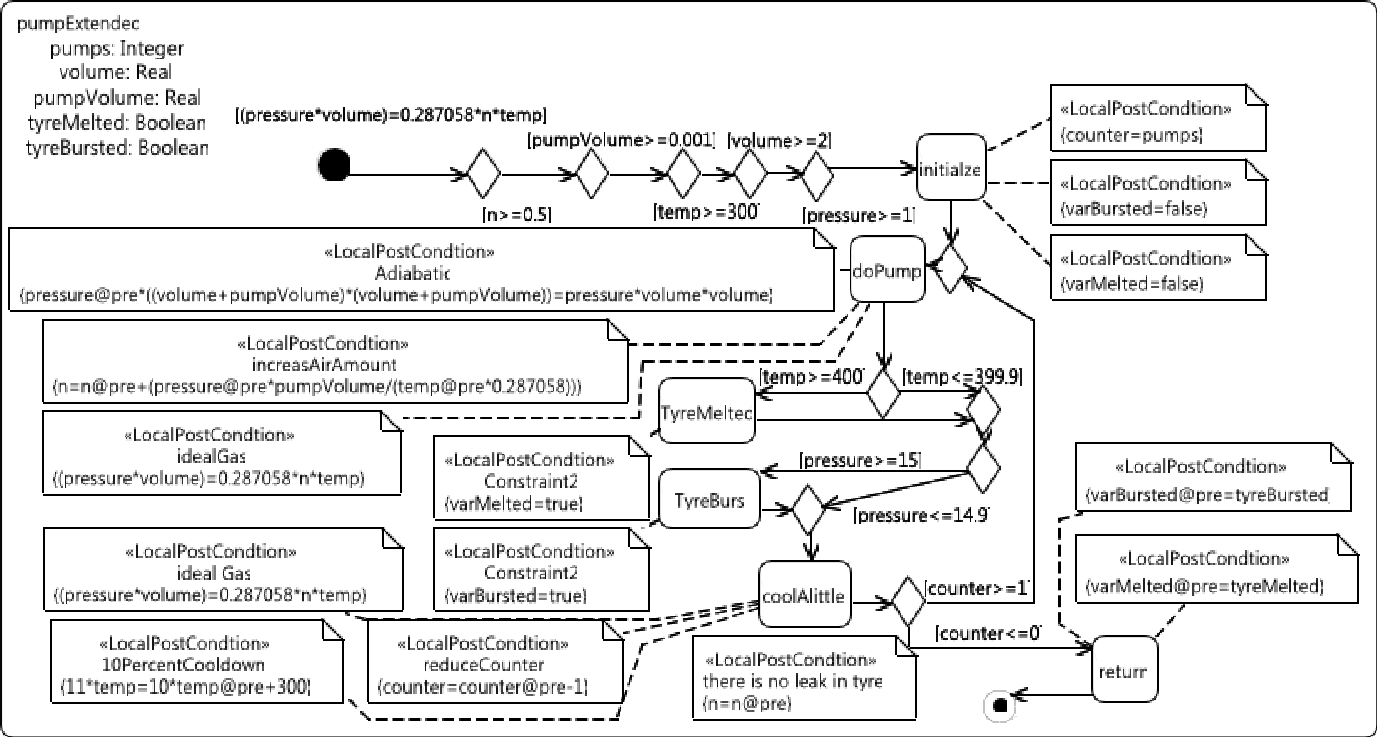
\includegraphics[width=\textwidth]{../Thesis/pics/pumpTyre.pdf}
\caption{Activity diagram with mixed integer non--linear constraints}
\label{fig:pumpTyre}
\end{figure}
Figure \ref{fig:pumpTyre} shows an activity diagram modelling the physical
process of pumping air into a tyre. The relations between \OCLVar{volume},
amount of air (\OCLVar{n}), \OCLVar{pressure}, and \OCLVar{temperature} are
described by the ideal gas equation. The equations for adiabatic compression of
air during one pump stroke states a non--convex relation between these physical
measures, consequently the resulting AMPL programs will be non--convex. Additionally we introduced the boolean variables \OCLVar{tyreExploded}
and \OCLVar{tyreMelted}, which will be set when the \OCLVar{pressure} or
\OCLVar{temperature} inside the tyre raised above a certain threshold. Moreover
we introduce an integer loop counter (\OCLVar{counter}) to count the number of
pump strokes. Consequently, the AMPL program is also a mixed integer problem.
\subsubsection{Runtime Measurement.}%
\begin{figure}%
\begin{center}%
\ref{myLegend}%
\end{center}%
\begin{tikzpicture}%
\begin{axis}[%
width=0.498\textwidth,
height=7cm,
legend columns=-1,
legend to name=myLegend,
ylabel={time $[s]$},
xlabel={maximum path length},
yticklabels={{0},{$0.1$},{$1$},{$10$},{$100$},{$10^3$},{$10^4$},{$10^5$}},
extra y ticks={3.6e12,2.592e14},
extra y tick labels={{1h},{3d}},
extra tick style={
        major grid style=black,
        tick align=outside,
        tick style=black
    },
minor x tick num=1,
ymajorgrids=true,
yminorgrids=true,
xmajorgrids=true,
xminorgrids=true,
ymode=log,
xmin=5,
xmax=75,
]
\addplot[dash pattern=on 4pt off 2pt on 1pt off 2pt,no markers] table[x=PATHSEARCH_MAX_PATHLENGTH,y=time(ns)]{../Thesis/Experiment-DATA/ExplodingTyres_5sec.csv};
\addlegendentry{5sec};
\addplot[dash pattern=on 7pt off 3pt,no markers] table[x=PATHSEARCH_MAX_PATHLENGTH,y=time(ns)]{../Thesis/Experiment-DATA/ExplodingTyres_10s.csv};
\addlegendentry{10sec};
\addplot[densely dotted,no markers] table[x=PATHSEARCH_MAX_PATHLENGTH,y=time(ns)]{../Thesis/Experiment-DATA/ExplodingTyres_20sec.csv};
\addlegendentry{20sec};
\addplot[loosely dashed,no markers] table[x=PATHSEARCH_MAX_PATHLENGTH,y=time(ns)]{../Thesis/Experiment-DATA/ExplodingTyres_60sec.csv};
\addlegendentry{60sec};
\addplot[densely dashed,no markers] table[x=PATHSEARCH_MAX_PATHLENGTH,y=time(ns)]{../Thesis/Experiment-DATA/ExplodingTyres_10min.csv};
\addlegendentry{10min};
\addplot[solid,no markers] table[x=PATHSEARCH_MAX_PATHLENGTH,y=time(ns)]{../Thesis/Experiment-DATA/ExplodingTyres_2h.csv};
\addlegendentry{2h};%
\end{axis}%
\end{tikzpicture}%
\begin{tikzpicture}%
\begin{axis}[%
width=0.498\textwidth,
height=7cm,
xlabel={maximum path length},
ylabel={number of test cases found},
minor x tick num=1,
minor y tick num=4,
ymajorgrids=true,
yminorgrids=true,
xmajorgrids=true,
xminorgrids=true,
xmin=35,
xmax=75,
]
\addplot[dash pattern=on 4pt off 2pt on 1pt off 2pt,no markers] table[x=PATHSEARCH_MAX_PATHLENGTH,y=PathsFound]{../Thesis/Experiment-DATA/ExplodingTyres_5sec.csv};
%\addlegendentry{5sec};
\addplot[dash pattern=on 7pt off 3pt,no markers] table[x=PATHSEARCH_MAX_PATHLENGTH,y=PathsFound]{../Thesis/Experiment-DATA/ExplodingTyres_10s.csv};
%\addlegendentry{10sec};
\addplot[densely dotted,no markers] table[x=PATHSEARCH_MAX_PATHLENGTH,y=PathsFound]{../Thesis/Experiment-DATA/ExplodingTyres_20sec.csv};
%\addlegendentry{20sec};
\addplot[loosely dashed,no markers] table[x=PATHSEARCH_MAX_PATHLENGTH,y=PathsFound]{../Thesis/Experiment-DATA/ExplodingTyres_60sec.csv};
%\addlegendentry{60sec};
\addplot[densely dashed,no markers] table[x=PATHSEARCH_MAX_PATHLENGTH,y=PathsFound]{../Thesis/Experiment-DATA/ExplodingTyres_10min.csv};
%\addlegendentry{10min};
\end{axis}%
\end{tikzpicture}%
\caption{Runtime consumed and test cases found for the tyre pump model%
%. We used Couenne as solver. The maximum path length and the solver time limit have been varied.
}%
\label{fig:ExplodingTyresRuntime}%
\end{figure}%
Mixed integer non--linear programs are in general undecidable. Consequently,
solvers might not halt on an MINLP instance. During test generation we need to
solve lots of MINLP instances. It is advisable to set a suitable time limit
after which the solver shall terminate and we assume the currently examined
control flow path as infeasible. For very small time limits test generation is
faster while for longer time limits chances to find a solution for a particular
MINLP instance are rising. In other words, when setting a larger time limit we
will certainly find a solution more often and thus generate more test cases but
the overall runtime will grow.

Figure~\ref{fig:ExplodingTyresRuntime} depicts the overall runtime of the
test generation for the \UMLType{Activity} from Figure~\ref{fig:pumpTyre}. We
used Couenne as solver for MINLP instances and varied the time limit to solve
one MINLP instance between 5 seconds and 10 minutes. The right hand side of
Figure~\ref{fig:ExplodingTyresRuntime} depicts the number of abstract test
cases for which we could find test data with the given solver time
limit. The number of abstract test cases grows exponentially with the maximum
path length and so does the overall computation time and the number of real test
cases.

Up to a path length of 30 all problem instances had been solved or found
infeasible after less than 10 seconds, thus the solver time limits did not make
a difference in the runtime or for the number of test cases found. Comparing the
runtime of our algorithm with different time limits for the maximum path length
of 60 we recognise that increasing the time limit from 20 seconds to 60 seconds
increased the overall runtime by a factor of 2.78 and generated 17 more real
test cases; those are 9.2\% more test cases. Increasing the time limit from 60
seconds to 600 seconds increased the overall runtime by a factor of 7.67 and
produced 11 additional test cases, which amounts to only 5.4\% more test cases.
We see that increasing the time limit for the solver massively increases the
overall runtime, but we gain only very few additional test cases for that and we
doubt that those additional test cases massively increase the quality of the
test suite. We therefore recommend using less than 20 seconds as solver time
limit for Couenne.
\subsubsection{Mutation Testing.}
We performed mutation testing with the test cases generated from the tyre pump
model. Although the tests were not exhaustive, they yield some interesting
results. In the model there is a loop and in every round the values for
\OCLVar{temperature}, \OCLVar{pressure}, amount of air (\OCLVar{n}) are updated
depending on the values of those measures before. Consequently, when one of the
calculations has a small error the error will be propagated to all three of
those measures and we see a great number of failed tests due to just one wrong
statement. Similarly, reordering of statements introduced huge errors in all
three measures. And finally, a sub--optimal calculation plans caused several
test cases to fail due to rounding errors. One might think that the C
expressions \verb$(10 * temp + 300) / 11$ and \verb$10 * temp / 11 + 300 / 11$
are equivalent. But the automatically generated test cases revealed that those
two expressions do not produce the same results.
\subsection{Case Study}
\label{sec:CaseStudy}
We tested our implementation on a model of the PAX call system from Airbus
Operations GmbH. Out of the model of the complete product we selected a large
activity diagram modelling the control flow of a function. The selected
\UMLType{Activity} contains 21 \UMLType{Actions}, 24 \UMLType{ControlNodes}, and
two \UMLType{LoopNodes}. Furthermore, there are eight \UMLType{DataStoreNodes}
representing function local variables. The branching conditions and the code
body of each \UMLType{Action} is given in C syntax. All assignments and
conditions consist of linear equations and inequalities only. All variables are
in the integer or boolean domain. Consequently, the constraint satisfaction
problem to be solved for test data generation is a mixed integer linear program.
The solvers Cplex and LPsolve are perfectly suitable for this kind of problem.
Couenne can also be used for this task.

The algorithm described in Section~\ref{sec:Algorithm} has several parameters.
We use this case study to evaluate the influence of those parameters on the
runtime. The examined parameters are the maximum path length, maximum amount of
test cases, unchecked steps, and the solver to use.
\subsubsection{Manual Adaptation.}
In order to generate C++ unit test code from the model using our Eclipse plug--in, 
manual pre--processing is necessary: import the model, add \UMLReference{guard}s and
\UMLReference{localPostcondition}s in OCL syntax, flatten the
\UMLType{LoopNodes}, and replace the \UMLType{DataStoreNodes} by
\UMLType{Properties}.

The model was provided as XMI export from Atego\textsuperscript{\textregistered}
Artisan Studio. Each modelling tool has its own implementation of the UML meta
model. Due to slight differences in the implementations it is not directly
possible to load an XMI file from Atego\textsuperscript{\textregistered} in
Eclipse. We manually removed some objects not recognised by Eclipse and
corrected some typing errors in the XMI file. Then we could load the XMI file
and browse the model with the Eclipse Modelling Framework.

Every \UMLType{Action} and \UMLReference{ControlFlow} contains C code snippets,
but no OCL constraints. We added
\UMLReference{guards} and \UMLReference{localPostconditions} reproducing the
semantics of the C code snippets contained in the original model.

The original model used local C struct variables modelled by the
\UMLType{DataStoreNodes} contained by the \UMLType{Activity}. Our implementation
can handle primitive data type variables modelled by the \UMLType{Property}
element. Consequently, we created one \UMLType{Property} per field of a struct
variable. The original model also used arrays. We emulated the behaviour of an
indexed collection by allowing all variables depending on an index to change to
an arbitrary value. This may produce wrong
behaviour but seemed good enough to evaluate the runtime of our algorithm.

The \UMLType{LoopNodes} contain further model elements in their
\UMLReference{bodyPart}. We connect those elements from the
\UMLReference{bodyPart} to additional \UMLType{ControlFlow}s and
\UMLType{ActivityNode}s emulating the counter loop semantic. The
\UMLType{LoopNode} is discarded and its augmented \UMLReference{bodyPart} is
directly embedded in the \UMLType{Activity}.

The function specifying which \UMLType{ControlFlow} to take after each
\UMLType{Action} is well--defined and defined over the complete domain.

\subsubsection{Runtime Measurement Results.}
We examine the influence of the used solver, the maximum path length, the
maximum number of test cases, and the unchecked steps on the runtime of our
algorithm. All runtime measurements have been performed with an
Intel\textsuperscript{\textregistered} Core\textsuperscript{\texttrademark} 2
Duo CPU.%
\paragraph{Different Solvers}%
% \begin{figure}%
% \begin{tikzpicture}%
% \begin{axis}[%
% width=0.59\textwidth,%
% height=7cm,%
% %legend columns=-1,
% %legend to name=solvers,
% legend style={at={(0.02,0.98)},anchor=north west},
% xlabel={maximum path length},
% ylabel={time $[s]$},
% yticklabels={0,{$1$},{$10$},{$100$},{$10^3$},{$10^4$},{$10^5$}},%
% extra y ticks={3.6e12,2.592e14},%
% extra y tick labels={{1h},{3d}},%
% extra tick style={
%         major grid style=black,
%         tick align=outside,
%         tick style=black
%     },
% minor x tick num=1,
% xmin=15,
% xmax=115,
% ymax=1e14,
% ymajorgrids=true,
% yminorgrids=true,
% xmajorgrids=true,
% xminorgrids=true,
% ymode=log,
% ]
% \addplot[loosely dashed] table[x=PATHSEARCH_MAX_PATHLENGTH,y=time(ns)] {../Thesis/Experiment-DATA/CaseStudyRuntimeCplex.csv};
% \addlegendentry{Cplex};
% \addplot[dash pattern=on 7pt off 4pt] table[x=PATHSEARCH_MAX_PATHLENGTH,y=time(ns)] {../Thesis/Experiment-DATA/CaseStudyRuntimeLPSolve.csv};
% \addlegendentry{LPsolve};
% \addplot[densely dashed] table[x=PATHSEARCH_MAX_PATHLENGTH,y=time(ns)] {../Thesis/Experiment-DATA/CaseStudyRuntimeCouenne.csv};
% \addlegendentry{Couenne};
% \addplot[densely dotted] table[x=PATHSEARCH_MAX_PATHLENGTH,y=time(ns)] {../Thesis/Experiment-DATA/CaseStudyRuntimeGecode.csv};
% \addlegendentry{GeCoDE};
% \addplot[solid] expression[no markers, domain=30:110]{2e7*1.12^(x)} node[pos=0.5,sloped,fill=white, below, opacity=1,text opacity=1] {$1.12 ^ {x}$} ;
% \end{axis}
% \end{tikzpicture}
% \begin{tikzpicture}
% \begin{axis}[
% width=0.39\textwidth,
% height=7cm,
% ylabel={number of test cases},
% xlabel={maximum path length},
% minor x tick num=4,
% ymajorgrids=true,
% yminorgrids=true,
% xmajorgrids=true,
% xminorgrids=true,
% ymode=log,
% ]
% \addplot[solid,mark=x] table[x=PATHSEARCH_MAX_PATHLENGTH,y=PathsFound]{../Thesis/Experiment-DATA/CaseStudyRuntimeLPSolve.csv};
% \addplot[color=black, style=dashed] expression[no markers, domain=30:100]{1.1 ^ (x)} 
% node[pos=0.5,sloped,fill=white, below, opacity=1,text opacity=1] {$1.1 ^ {x}$}
% ;
% \end{axis}
% \end{tikzpicture}
% %\end{center}
% \caption{Runtime of our algorithm applied to the case study%
% %. We measured the runtime with different solvers and varied the maximum path length. The runtime as well as the amount of test cases grow exponentially with the maximum path length.%
% }%
% \label{fig:RuntimeExperimentsSolvers}%
% \end{figure}%
We measured the runtime with different solvers and found that the runtime grows
almost exponentially with the maximum path length: It doubles when the
maximum path length increases by $6$-$7$. The solvers LPsolve, Cplex, and GeCoDE
are equally fast. The solver Couenne consumed about three times the runtime
consumed using LPsolve. This might be because Couenne is actually suitable for
the much more general mathematical problem of mixed integer non--linear
programming; it is not perfectly specialized for mixed integer linear
programming.

The case study model contains only constraints that are instances of mixed
integer linear programming and, therefore, the solvers succeed to find test data
for every feasible path. Consequently, our algorithm will produce one test case
for every feasible path. The number of test cases grows equally exponential with
the maximum path length as the runtime. For a maximum path length of 110 a total
of 12,850,000 linear programs had to be solved to find 83,000 sets of test data.
The fastest solver, LPSolve, took only 13 hours for this task. This makes 275
solved problems per second and among them 1.8 produced actual test data.
\paragraph{Unchecked Steps}%
\begin{figure}
\begin{center}
\begin{tikzpicture}
\begin{axis}[
width=0.6\textwidth,
height=7cm,
legend style={legend columns=1,at={(1.02,0.98)},anchor=north west},
xlabel={unchecked steps},
xmax=15,
ylabel={time $[s]$},
yticklabels={{$1$},{$10$},{$100$},{$10^3$},{$10^4$},{$10^5$}},
extra y ticks={3.6e12,2.592e14},
extra y tick labels={{1h},{3d}},
extra tick style={
        major grid style=black,
        tick align=outside,
        tick style=black
    },
minor x tick num=1,
ymajorgrids=true,
yminorgrids=true,
xmajorgrids=true,
xminorgrids=true,
ymode=log,
]
\addlegendimage{empty legend}
\addlegendentry{maximum path length}
\addplot[dash pattern=on 4pt off 2pt on 1pt off 2pt] table[x=PATHSEARCH_UNCHECKED_STEPS,y=time(ns)]{../Thesis/Experiment-DATA/CaseStudyUncheckedSteps90.csv};
\addlegendentry{90};
\addplot[dash pattern=on 7pt off 2 on 1 off 2] table[x=PATHSEARCH_UNCHECKED_STEPS,y=time(ns)]{../Thesis/Experiment-DATA/CaseStudyUncheckedSteps80.csv};
\addlegendentry{80};
\addplot[dash pattern=on 7pt off 3pt] table[x=PATHSEARCH_UNCHECKED_STEPS,y=time(ns);]{../Thesis/Experiment-DATA/CaseStudyUncheckedSteps70.csv};
\addlegendentry{70};
\addplot[densely dashed] table[x=PATHSEARCH_UNCHECKED_STEPS,y=time(ns);]{../Thesis/Experiment-DATA/CaseStudyUncheckedSteps60.csv};
\addlegendentry{60};
\addplot[loosely dashed] table[x=PATHSEARCH_UNCHECKED_STEPS,y=time(ns)]{../Thesis/Experiment-DATA/CaseStudyUncheckedSteps50.csv};
\addlegendentry{50};\addplot[solid] table[x=PATHSEARCH_UNCHECKED_STEPS,y={time(ns)}]{../Thesis/Experiment-DATA/CaseStudyUncheckedSteps40.csv};
\addlegendentry{40};
\end{axis}
\end{tikzpicture}
\end{center}
\caption{Runtime of our implementation depending on the unchecked steps%
%. The experiment has been performed with Cplex as solver for different maximum path lengths
}%
\label{fig:RuntimeUncheckedSteps}%
\end{figure}%
In Figure~\ref{fig:RuntimeUncheckedSteps}, we plotted the overall runtime of our
algorithm depending on the unchecked steps of the early infeasible path
elimination. We used Cplex as solver for this experiment and repeated the
experiment for different maximum path lengths. In the plots we see, up to a
maximum path length of 50 it is not beneficial to use early infeasible path
elimination when generating test cases for the case study model. With longer
maximum path lengths the impact of well configured early infeasible path
elimination grows. For a maximum path length of 90 our algorithm configured with
the optimal value for the unchecked steps parameter takes less than one hour to
generate all test cases, while it takes several days when unchecked steps is set
to 5 or 6.%
\paragraph{Maximum Amount of Test Cases}
\begin{figure}
\begin{tikzpicture}
\begin{axis}[
width=0.49\textwidth,
height=7cm,
xlabel={number of test cases},
ylabel={time $[s]$},
scaled y ticks = false,
% xtick scale label code/.code={\xdef\xtickscale{#1}}, 
yticklabels={0,{$1$},{$10$},{$100$},{$10^3$},{$10^4$},{$10^5$}},
extra y ticks={3.6e12,2.592e14},
extra y tick labels={{1h},{3d}},
extra tick style={
        major grid style=black,
        tick align=outside,
        tick style=black
    },
minor x tick num=1,
ymajorgrids=true,
yminorgrids=true,
xmajorgrids=true,
xminorgrids=true,
ymode=log,
xmode=log,
] 
\addplot[solid,mark=x] table[x=PathsFound,y=time(ns)]{../Thesis/Experiment-DATA/CaseStudyRuntimeLPSolve.csv};
\addplot[color=black, style=dashed] expression[no markers, domain=1e2:1e5]{(2e7) * x}
node [pos=0.7,below,sloped,fill=white,opacity=0.85,text opacity=1] {$x^1$} 
;
\addplot[color=black, style=dashed] expression[no markers, domain=1e2:1e5]{(4e6) * x ^ (1.45)} 
node [pos=0.9,sloped,above,fill=white,opacity=0.85,text opacity=1] {$x^{1.45}$} 
;
\addplot[color=black, style=dashed] expression[no markers, domain=1e2:1e4]{(6e5) * x ^ (2)} 
node [pos=0.7,sloped,above,fill=white,opacity=0.85,text opacity=1] {$x^{2}$} 
;
\end{axis}
\end{tikzpicture}
\begin{tikzpicture}
\begin{axis}[
width=0.49\textwidth,
height=7cm,
xlabel={maximum amount of test cases},
ylabel={time $[s]$},
legend style={legend columns=1,at={(0.02,0.98)},anchor=north west},
scaled y ticks = false,
yticklabels={{0},{0},{$2\cdot 10^{3}$},{ },{$6\cdot 10^{3}$},{$8\cdot 10^{3}$}},
extra y ticks={3.6e12,2.592e14},
extra y tick labels={{1h},{3d}},
extra tick style={
        major grid style=black,
        tick align=outside,
        tick style=black
    },
minor x tick num=1,
minor y tick num=4,
ymajorgrids=true,
yminorgrids=true,
xmajorgrids=true,
xminorgrids=true,
xmin=500,
xmax=9500,
] 
\addplot[dotted,mark=x] table[x=PathsFound,y=time(ns)]{../Thesis/Experiment-DATA/CaseStudyRuntimeCplex.csv};
\addlegendentry{DFS}
\addplot[solid,mark=x] table[x=PathsFound,y=time(ns)]{../Thesis/Experiment-DATA/CaseStudyRuntimeBFS.csv};
\addlegendentry{BFS}
\end{axis}%
\end{tikzpicture}%
\caption{Runtime depending on the number of test cases. Left: depth--first search. Right: breadth--first search}
\label{fig:RuntimeExperimentsData}
\end{figure}
The runtime as well as the number of abstract test cases grows exponentially
with the maximum path length. The quotient of runtime and generated test cases
grows polynomially. To illustrate that, we plotted the runtime of our algorithm
against the number of test cases in Figure~\ref{fig:RuntimeExperimentsData}. 

For the plot of the left we did not use the parameter maximum amount of test
cases but plotted the number of test cases actually found against the runtime of
our algorithm using different values for maximum path length. It is logarithmic
on both axes and we can see that the runtime grows with an exponent of $1.45$.

Depth--first search without limit on the maximum path length but with a limit on
the number of test cases, would not produce useful test cases. All generated
abstract test cases would over and over share very long common sub--paths and
some \UMLType{ControlFlow}s would not be checked at all. Therefore, we
implemented a breadth--first search--based alternative to the algorithm
explained in Section~\ref{sec:InfeasiblePathElimination}. We use this
alternative to evaluate the effect of the maximum amount of test cases on the
runtime.

In Figure~\ref{fig:RuntimeExperimentsData}, we plot on the right the runtime of
our algorithm with breadth--first search and Cplex as solver. The dotted line
shows a small section of the left plot. As we can see breadth--first search is
considerably slower than depth--first search. The reason for that is that
breadth--first search can not make such a good use of the warm start
capabilities of the solvers as depth--first search can. In depth--first search,
usually only a small amount of the constraints change between two subsequent
solver invocations. For breadth--first search it will happen several times
during infeasible path elimination that all constraints have changed between two
subsequent solver invocations. Furthermore, we see that the generation of 9,000
test cases took only slightly longer than the generation of 8,000 test cases. We
can not explain this last effect.
\paragraph{Boundary Value Analysis}
\label{sec:caseStudyBoundaryValues}
\begin{figure}
\begin{center}
\begin{tikzpicture}
\begin{axis}[
width=0.59\textwidth,
height=7cm,
%title={Influence of boundary value analysis},
legend style={at={(0.02,0.98)},anchor=north west},
ylabel={time $[s]$},
xlabel={maximum path length},
%ytick={1e8,1e10,1e12,1e14},
yticklabels={0,{1},{10},{100},{$10^3$},{$10^4$},{$10^5$}},
extra y ticks={3.6e12,2.592e14},
extra y tick labels={{1h},{3d}},
extra tick style={
        major grid style=black,
        tick align=outside,
        tick style=black
    },
ymajorgrids=true,
yminorgrids=true,
xmajorgrids=true,
xminorgrids=true,
ymode=log,
]
\addplot[dotted,mark=x] table[x=PATHSEARCH_MAX_PATHLENGTH,y=time(ns)]{../Thesis/Experiment-DATA/CaseStudyRuntimeBoundaryValues.csv};
\addlegendentry{enabled};
\addplot[dashed,mark=x] table[x=PATHSEARCH_MAX_PATHLENGTH,y=time(ns)]{../Thesis/Experiment-DATA/CaseStudyRuntimeNoBoundaryValues.csv};
\addlegendentry{disabled}
\end{axis}%
\end{tikzpicture}%
\end{center}%
\caption{Comparison of runtime with boundary value analysis enabled and disabled}%
\label{fig:RuntimeBoundaryValue}%
\end{figure}%
Finally, we analysed the impact of boundary value analysis on the runtime of our
implementation. As explained in Section~\ref{sec:BoundaryValueAnalysis}, an
additional objective has been added in the AMPL program. We minimise the sum of
all initialisation values. In Figure~\ref{fig:RuntimeBoundaryValue}, we show the
runtime of our algorithm depending on the maximum path length. We use LPsolve as
solver. The runtime with boundary value analysis and the runtime without
boundary value analysis are plotted. The plot clearly shows that it does not
make a difference at all for the runtime whether we generate boundary test data
or just any test data.

This result is plausible because the number of solver invocations where really a
boundary value analysis is performed is small compared to the number of total
solver calls. For example, for a maximum path length of $70$ there are $1568$
test cases. The solver performs the optimisation only for them. On the other
hand, there are $35044$ solver invocations in total including those that
recognise a control flow path as infeasible. Consequently, only $4.5\%$ of all
solver invocations are actually performing some extra work. For larger maximum
path lengths this fraction is declining further.

We definitely recommend to use this feature for mixed integer linear programs in
practice because it really comes at no cost, and one can use this feature to
generate test data at two or more different boundaries of the feasible set and
generate multiple test cases for one control flow path that check all path
conditions for the control flow path.

\subsection{Limitations}
A natural limitation for constraint-solver-based test data generation is
decidability. There is no effective method to generate variable instantiations
that satisfy an arbitrary mathematical term and heuristics may not come to a halt on
some problem instances.
Currently, we support only a subset of the UML activity modelling
elements. For instance, hierarchical activity diagrams and concurrency are currently not
supported. 
%Also support for complex data types as well as OCL collections have been neglected.
Finally, our path search algorithm currently suffers
from combinatorial explosion. Generating test cases that adhere to a feasible
coverage criterion like, e.g., control flow coverage, would avert this problem.

\section{Summary and Recommendation}%
\label{sec:Recommendation}%
In this paper, we presented an efficient way to integrate state--of--the--art constraint
solvers into a model--based testing tool. Depending on the specific needs of the
modeller, a variety of constraints can be used in the model. 
We showed that the automatic test data generation is especially
fast when constraints are specified in terms of a decidable theory and solved
with an optimised solver. On the other hand we 
generated test data for models whose constraints are formulated as instances of
an undecidable problem like, e.g., mixed integer non--linear programming.
Although our approach makes it possible to generate test data for
models with undecidable constraints, this can be very time consuming.
Furthermore, it is not guaranteed that existing test data will be found. 
We recommend restricting
oneself to linear inequalities or another decidable constraint formulation.

We have presented a concept for early infeasible path elimination during
generation of abstract test cases and examined its impact on the overall runtime
of our algorithm. Using early infeasible path elimination with two unchecked
steps massively reduces the runtime of our algorithm.

Finally, we showed that the presented approach allows to steer the
generation of test data in a way that boundary values are produced with no
additional effort. It is common knowledge that the use of boundary values as
test data tends to trigger existing bugs with a higher probability. Thus we
improved the quality of the generated test cases with little additional effort.%

\bibliographystyle{splncs}%
\bibliography{../Thesis/bibtex}%
\end{document}